\documentclass{article}

\usepackage[ddmmyyyy]{datetime} 
\usepackage{caption}
%\usepackage[backend=biber, style=authoryear]{biblatex}
\usepackage[backend=bibtex8, style=authoryear]{biblatex}
\usepackage{hyperref}
\usepackage{amsmath}
\usepackage{graphicx}
\usepackage[font=small,labelfont=bf]{caption}

\addbibresource{Report.bib} % BibLaTeX bibliography file 

\begin{document}
	\title{Report Information Visualisation}
	\author{Oruç Kaplan; Ward Van den Bossche; Axel Daniel Vuillaume \& Laurens Devloo}
	\maketitle
	\tableofcontents
	\newpage
	
	\section{Data}
	
	\subsection{Dataset}
	
	This project will use two different datasets
	
	\begin{itemize}
		\item \href{https://www.kaggle.com/datasets/fronkongames/steam-games-dataset/code}{Steam Game Data}
		\item\href{https://developer.valvesoftware.com/wiki/Steam_Web_API}{Steam API for user information}
	\end{itemize}
	
	The steam game dataset contains data about games received from the Steam API and Steam Spy. The contained columns are name of the game, the release date, the amount of DLC for the game, a short description of the game, is the game is on Linux, Windows or on Mac, a metacritic score, the amount of achievements the game has, user score the amount of negative reviews and positive reviews, an email address for help, an average playtime and the amount of owners of the game. This data is found in the JSON-file \textit{/Data/games.json}.\\
	\\
	The second dataset is user information acquired from the Steam API. This dataset will contain the data about a given Steam user. This information includes the games he plays and the user-profiles of his friends.
	
	\subsection{Target User}
	
	The target users are gamers, both casual as experienced ones. The general idea is for gamers to get some interesting game recommendations, after having explored their own tastes through our app and viewing statistics about the full steam game dataset. The site will be able to do three things: The first is to give general information about the games such as how many games are supported by a country's official language, the top 5 games and constitution of the dataset per genre. The second thing that is possible for the user is to get a better insight into their own gaming-behaviour. An example of this would be seeing their own most played games per genre, the amount of hours played and the achievements acquired for these games. The third feature is to get a recommendation, for instance by comparing the stats of the user's owned games with their friend's games.
	
	\newpage
	
	\section{Preprocessing}
	
	In order to do the preprocessing please read the README.
	
	\subsection{Data Cleaning}
	
	The Steam games dataset as it stands needs more work in order to be usable in visualisations. This preprocessing will consist out of deleting unused columns, cleaning cells that point to outliers and dividing the certain columns into separate files for easier and faster access. The code in the Jupyter notebook, up until the custom score part, was heavily inspired by a publicly available kaggle notebook by \autocite{CLARAMUNT}. However, certain modifications were made to better align with our vision.\\
	\\
	As the dataset has more then 40 columns this means that we have to filter out the columns in order to end up with only those that will be used. The columns that will be deleted are: \texttt{packages}, \texttt{screenshots}, \texttt{movies}, \texttt{score\_rank}, \texttt{header\_image}, \texttt{reviews}, \texttt{website}, \texttt{support\_url}, \texttt{notes}, \texttt{support\_email}, \texttt{median\_playtime\_2weeks}, \texttt{required\_age}, \texttt{metacritic\_url}, \texttt{detailed\_description}, \texttt{about\_the\_game} and \texttt{average\_playtime\_2week}.\\
	These columns were deleted because they were either unfit for visualization as they were things like urls, notes, descriptions and emails, or the columns contained data that was not usable in our specific use case as is the case with \texttt{average\_playtime\_2weeks}.\\
	\\
	After this we delete outliers or values that seem to show useless rows. The first way we achieve this is by deleting all games with no sales. To do this we look where the \texttt{estimated\_owners} column equals \texttt{0-0} and delete the accompanying rows.\\
	Besides this we also see that some games have no reviews or categories. These are considered to be developer tests and so can be deleted.\\
	If we look at the distribution of the prices we can see that most of them are under 200\$. We have 1 game of 999\$, in order to not to affect the rest of the data this outlier is also removed from the dataset.\\
	\\
	The column \texttt{estimated\_owners} is a range between the minimal amount of owners and the maximum. In order for easier handling, this is split into 2 different columns: the \texttt{min\_owners} and the \texttt{max\_owners}.\\
	\\
	To conclude we look at the \texttt{median\_playtime\_forever} column. If these values are above 60,000 this would mean that over half of the playerbase would have played more than 1,000 hours. This would not be very realistic and so these values will be set to 0 in order to prevent skewing the data. Entries with this amount of hours will mostly not be games, but more so overlays or pieces of software that are running in the background.\\
	\\
	All this cleaned data will be saved to the file \textit{/Data/cleaned\_games.csv}.\\
	\\
	The dataset still contains columns such as \texttt{categories} or \texttt{tags} that consist out of a lists of values. In order to improve our performance we shall convert these fields into a separate table linked to the main table using \texttt{app\_id} as foreign key.\\
	In this implementation we went with the approach that only the games with non-empty lists will be included in the new table. Each new item of the list will be a new row in the table, making the primary key the combination of \texttt{app\_id} and value of the list.\\
	These different tables are saved to the files \textit{/Data/[column-name].csv}\\
	\\
	We can see in the dataset that there are quite a lot of different types of score columns. In order to combine them for recommending purposes, we make a custom score column named \texttt{score}.\\
	For this custom score we take into account the columns: \texttt{price}, \texttt{metacritic\_score}, \texttt{positive}, \texttt{negative} and \texttt{median\_playtime\_forever}.\\
	The first thing that has to happen is a normalization of the columns so neither of them affects the end result more. For the price we would like a range between $\left[0;1\right]$.
	
	$$normalised\_price = \frac{1}{\sqrt{\max{\left(price, 1\right)}}}$$
	
	Notice that we favor lower prices. The max function will prevent divisions by 0.\\
	The following 2 normalized scores are the \texttt{metacritic\_score} and \texttt{positive\_ratio}. Following these formulas:
	
	\begin{align}
		metacritic\_score\_normalized &= \frac{metacritic\_score}{\max{\left(metacritic\_score\right)}} \\
		positive\_ratio &= \frac{positive}{\max{\left(positive + negative, 1\right)}}
	\end{align}
	
	The total review is a good indicator of how many people bought the game, so this term effectively serves as a "amount of sales" score. The purpose of this is to filter out games with very few reviews, where review rating could easily be skewed to be overly positive or negative.
	
	\begin{align}
		total\_reviews\_normalized &= \frac{positive + negative}{\max{\left(positive + negative\right)}}\\
		median\_playtime\_forever\_normalized &= \frac{median\_playtime\_forever}{\max{\left(median\_playtime\_forever\right)}}	
	\end{align}
		
	After normalizing all the data we can give a weight to each column. The given weights are \texttt{price\_weight} = 0, \texttt{metacritic\_score\_weight} = 0, \texttt{positive\_ratio\_weight} = 1.5 as a high positive ratio is a good indicator of a game's quality. \texttt{total\_reviews\_weight} = 2.5 in order to favor more bought games. To end the \texttt{median\_playtime\_forever\_weight} = 0 as median playtime is more easily manipulated in lower selling games. 
    We tie everything together by giving following formula for the custom score:
	
	\begin{align}
		score = &price\_normalized\cdot price\_weight\\
		 &+ metacritic\_score\_normalized\cdot metacritic\_score\_weight\\
		 &+ positive\_ratio\cdot positive\_ratio\_weight\\
		 &+ total\_reviews\_normalized\cdot total\_reviews\_weight\\
		 &+ median\_playtime\_forever\_normalized\cdot median\_playtime\_forever\_weight
	\end{align}
	
    Note that a weight value of 0 means that category wasn't used to calculate the score, effectively making a score that only combines "total reviews" and "positive review percentage" in our current implementation. We found that this caused the bubble chart to recommend games that best aligned with our vision of what most users would find important. However, we left the full formula in the notebook to showcase the idea of the score column and for possible future reference.
    
	All the code for data cleaning can be found in the jupyter notebook: \textit{/utils/steam-games-data-transformation.ipynb}
	
	\subsection{Group By}
	
	We have a couple of columns that can be used to group by such as languages, categories, genres, etc. Due to the size of the dataset it takes too long to compute the grouped by information on the fly. In order to keep the wait times low we pre-calculate all this information in the preprocessing phase of the project.\\
	All the numeric values will be summed over all the array-like columns such as \texttt{categories}, \texttt{full\_audio\_languages}, \texttt{genres} and \texttt{supported\_languages}. The new tables will be written to \textit{/Data/[name-column]\_grouped\_by.csv}.\\
	\\
	This is all handled by the \textit{/utils/data\_processing.py} file
	\newpage
	
	\section{Visualisation}
	\subsection{Home}

	\subsubsection{Gauges}
	
	\begin{itemize}
		\item Goal : See what the percentage of positive reviews are for games supported by the top 3 languages.
		\item Data : Aggregated data over the languages and summing the positive reviews. In order to get the percentages.
		\item Design and choice : Choose a black-white hue in order to always be clearly visible.
		\item Implementation : An indicator plot with number.
		\item Code file : \textit{gauge.py}
	\end{itemize}
	
    \subsubsection{Sunburst graph}
    \begin{itemize}
        \item Goal : View the most popular game categories based on the time spent by players.
        \item Data : Get the games, the categories and developer from the dataset.
        \item Features/Interaction : Click on a part to zoom in to see the developer or games more clearly. You can hover over a box to see the children or parents and the total average playtime. We added a button to hide the single player mode because the single player categories take up the most important part of the graph. Additionally, I added a slider to control how many games you want to see based on average playtime.
        \item Design and choice : Choose a sunburst to see the children better and compare play times more easily.
        \item Implementation : A sunburst chart with game, developer and categories by time spent.
        \item Code file : \textit{sunburst.py}
    \end{itemize}
    
    \subsubsection{World Map Graph}
    \begin{itemize}
        \item Goal : See the number of games depending on the languages supported.
        \item Data : Get data on supported languages and assign a country for each language.
        \item Features/Interaction : You can zoom in and out if you want to search for a specific country. By hovering over the country, you can see the name of the most played game in the country and their average playing time.
        \item Design and choice : Choose a green gradient to be clear.
        \item Implementation : A Choropleth chart with supported languages.
        \item Code file : \textit{map.py}
    \end{itemize}
    
    \subsubsection{Line Graph}
    \begin{itemize}
        \item Goal : Compare different data from the dataset.
        \item Data : Get price, metacritic\_score, user\_score, average\_playtime\_forever, score of the data set.
        \item Features/Interaction : Using a drop-down list, you can choose the x and y axes to compare the data you want to see. On hover, you can see the game name and the x and y values.
        \item Implementation : A line chart with x and y values from the drop-down list.
        \item Improvement : Create an entry to choose the X axis scale.
        \item Code file : \textit{graph.py}
    \end{itemize}

	\subsection{Profile}
    
   	\subsubsection{User Playtimes}
   	
        \paragraph{Stacked Barchart}
    
        \begin{itemize}
           \item Goal : Show how the user's games are distributed across different genres. Giving a quick overview of which games are played most, and what genre they belong to.
           \item Data : Playtimes from the user's game library, game name and genres acquired from matching app ids of the steam API with their respective games in the steam games dataset.
           \item Features/Interaction : A game slider underneath the graph makes it possible to add games amounts in increasing order of playtime, which makes it so the user can still view every item by adjusting the slider accordingly. Clicking on a genre in the legend makes it possible to show/hide a genre, alternatively you can double-click a genre to isolate it on the graph. Clicking a game on the graph updates 2 other graphs: the genre playtime barchart (on the right) and the achievement timeline chart (below the graph).
           \item Design and choice : We opted for a stacked barchart because it's a good way to get a quick overview of the playtime distribution over a user's library, this chart isn't meant to show detailed information. Considering there's only 33 unique genres in the games dataset, even in extreme cases where a user owns a game in every genre, the stacked barchart should still be able to serve it's purpose. The games slider underneath also helps in this regard, to gradually explore the games library. The genres are distinct colors, if the user has a large game library this means we might violate the 12-bin rule for colors. However, except for generating the legend on the right with plotly express, the colors mostly serve to differentiate the different bars. This design choice makes more sense when you consider that we were planning to link the colors on the genre chart (on the right) to the clicked genre on this stacked barchart. 
           \item Implementation : By matching the app ids acquired from the steam API to the ones in our steam games dataset, we easily find the related games. The playtimes we get straight from the API, and we display them in hours played. There's usually multiple genres associated with a single game, we didn't find a surefire way to pick the "most fitting" genre for a game, so we ended up picking a random one each time, to prevent them from all appearing in the same bar. 
           \item Code file : \textit{user\_playtime\_bar\_chart.py}, (function name: \textit{playtime\_per\_genre})
        \end{itemize}
        
        \paragraph{Horizontal barchart}
        
        \begin{itemize}
            \item Goal : Show all playtimes of the user's games in descending order of a single genre.
            \item Data : "Clickdata" relating to the clicked game on the stacked barchart, this is only used to extract the genre. Playtimes from the user's game library, filtered by genre.
            \item Features/Interaction : A simple horizontal barchart without interaction capabilities, on hover it shows the playtime of the game in hours.
            \item Design and choice : Considering the cluttered nature of the stacked barchart, combined with the fact that each game possibly belongs to multiple genres. We decided to add a more detailed horizontal barchart to get a closer look at the playtimes of a specific genre. 
            \item Implementation : By clicking on a game in the stacked barchart, a callback is triggered which passes on the "clickdata. We extract from this the genre of the clicked game and display all games in this genre with their respective playtimes, in descending order of playtime.
            \item Code file : \textit{user\_playtime\_bar\_chart.py}, (function name: \textit{playtime\_games\_per\_genre})
        \end{itemize}
        
    \subsubsection{Achievement timeline}
    
    \begin{itemize}
        \item Goal : Show achievements in ascending order of date acquired, on the x-axis, with the rarity of the achievement on the y-axis.
        \item Data : "Clickdata" resulting from clicking on a game in the stacked barchart. From this we extract the app id, by way of which we can acquire the achievement data from the steam API.
        \item Design and choice : This chart is a scatterplot where each achievement is represented by a symbol on the plot. Both shape and color channels are used to encode an achievement tier, there are 4 tiers based on the rarity of the achievement. We decided to use both color and shape because we had both channels available, and this way colorblind people are accounted for. On hover the full unlocktime and name of the achievement are displayed, as well as it's rarity percentage (global percent of people that have this achievement). If you double click an achievement tier in the legend, you can isolate that tier on the graph. We decided not to connect the dots as this would only clutter the graph more.
        \item Implementation : By clicking on a game in the stacked barchart, a callback is triggered which passes on the "clickdata". We extract from this the appid of the clicked game and ask the steam API for user's achievements of this game. After that we call the API again to get the global data for the achievements, add a new column to assign the 4 tiers based on global achievement percentage and encode all this data in our scatterplot.
        \item Code file : \textit{achievement\_chart.py}
    \end{itemize}
    
	\subsection{Recommender}
    
	\subsubsection{User Vs Friends Panel}
	
	The aim of this visualisation is to compare our tastes with those of our friends. To do this, it consists of two Spider Graphs, one for yourself and one for the selected friend, as well as two graphs (one for each) that appear in the centre, listing the top 5 games for the category/genre selected in the spider graph. The code for this visualisation can be found in \textit{user\_vs\_friends\_panel.py} the file \textit{hexagon.py} and \textit{top\_games\_forUVFpanel.py}.

	\paragraph{Spider Graphs}
	
	\begin{itemize}
		\item Goal : Show the user's preferences in terms of categories/genres by comparing the total playtime of the games in each category/genre and the total number of games played in each category/genre.
		\item Data : Get the games, genre and categories from the dataset and the user's playtime and number of games played from the Steam API.
		\item Features/Interaction : You can choose between the categories and genres of the games. You can change the number of categories/genres displayed by choosing the number of sides of the spider graph (it will show first the most played categories/genres). Hovering to get the number of games played and the total playtime in hours for each label (with a legend). Clicking on a label will show the top 5 games in this category/genre in the center graph. You can select a friend to compare your preferences of your top genre/categories to his preferences for the same genre/categories you like.
		\item Menu : Disposition on the top left, except for the friend selector which is above his spider graph (which makes more sense).
		\item Design and choice : The user and the friend are in disctinct colors, blueish for the user and redish for the friend to make clear distinction. The user and friend infos are in distinct spidergraph because the goal is to see the tastes by looking to the ratio between the playtime and the owned games per genre/category in each spidergraph. This also avoid having too much information in one graph and better for colorblindness and black/white since tranparency is envolved in the colors.
		\item Implementation : Since the radar charts are a bit limited in Ploty, we decided to do a custom implemented spider graph made with a scatter plot and lines between the points (a little bit risky).
		\item Code file : \textit{hexagon.py}
	\end{itemize}

	\paragraph{Center Graphs}
	
	\begin{itemize}
		\item Goal : Show the top 5 games in the selected category/genre for the user and the friend in order to see what games are the most played by our friend in the same category/genre in order to get some inspiration.
		\item Data : Get the games from the dataset and the user's playtime from the Steam API.
		\item Features/Interaction : Hovering to get the playtime in hours for each game.
		\item Menu : The spider graphs labels (whatever the user or the friend) will act as a menu to select the category/genre to display the top 5 games.
		\item Design and choice : The user and the friend are in disctinct colors, blueish for the user and redish for the friend to make clear distinction again. \texttt{The scales for the playtime} are not the same for two reasons: first because of the goal of the graph and second because a huge difference in playtime between the user and the friend would make the user's playtime unreadable (maybe a synchronized selection between the two graphs could be pertinent here (as saw in the Exercices Sessions with the lasso) but didn't have the time to implement it).
		\item Implementation : A simple bar chart with the top 5 games for the selected category/genre.
		\item Code file : \textit{top\_games\_forUVFpanel.py}
	\end{itemize}
	
	\subsubsection{Bubble Chart Recommendations}
	
	\begin{itemize}
		\item Goal : Recommend the user 5 games he doesn't own, for each of his most played genres.
		\item Data : User's game playtimes from the api, games and genres data from the dataset, score column to decide on the best games.
		\item Features/Interaction : Hovering over a bubble to get details about the game (name, price, genre, positive reviews, total reviews), drag across the graph to focus on a certain price-range, (double) click on a genre in the legend to show/hide games of that genre. 
		\item Design and choice : Each color represents a different genre, since only the 8 most played genres are shown, it adheres to the 12-color rule. The size of the bubble represents the total reviews of the game, which is a good approximation of the popularity. The bigger the bubble, the more popular the game. The x-axis represents the price of the game in US dollars, the y-axis represents the positive review percentage of the game. The graph takes up the whole width of the page, as the scarcity of visualizations on the recommender tab allowed for this.
		\item Implementation : The implementation is quite straightforward, for each genre the top 5 games are selected based on the score column mentioned in the preprocessing step.
		\item Code file : \textit{bubble\_chart.py}
	\end{itemize}
	
	\newpage

	\section{Evaluation}
	
	For the evaluation of the system we have asked Experts (target users) to use our site and share their experience with us.\\
	\\ 
	To do this we have used the UEQ V12 questionnaire. 26 questions were asked where for each a number between 1 and 7 have to be filled in. Each question can be put into on of 6 categories: Attractiveness, Perspicuity, Efficiency, Dependability, Stimulation and novelty. The questionnaire is setup so that it is also tested if the person filling in the questions is paying attention are not.\\
	\\
	\begin{figure}[h]
		\centering
		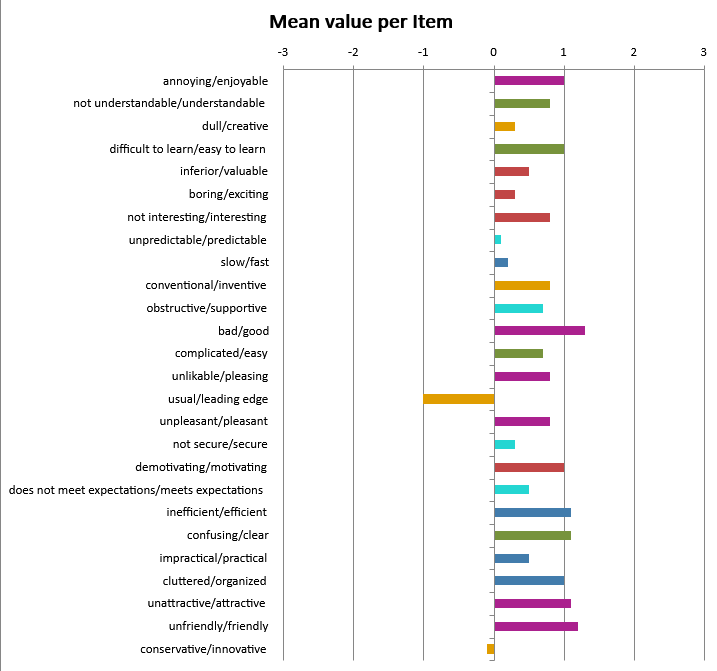
\includegraphics[width=\linewidth]{./Screenshots/Mean_value_per_item.png}
		\captionof{figure}{The results for each question}
		\label{fig:mean_value}
	\end{figure}
	\par
	
	As to be seen on figure \ref{fig:mean_value} all answers tend towards the "Positive" only those questions informing about Novelty tend toward the more conservative/usual side of the spectrum.\\
	This is a good result as we want to focus more on the other aspects as ease of use and reliability of the system.\\
	
	\begin{figure}[h]
		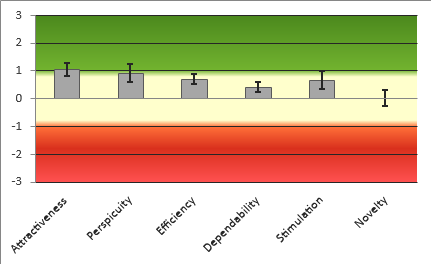
\includegraphics[width=\linewidth]{./Screenshots/Evaluation_result.png}
		\captionof{figure}{The results of the different questions divided in categories}
		\label{fig:evaluation_result}
	\end{figure}
	\par
	
	The results of figure \ref{fig:evaluation_result} give the average over the different categories with error bars. In here we see the same tendency that all the results are to the positive side and that only novelty is doing less so. Our best performing measure is "Attractiveness" with a mean of 1.03. The worst measure is as aspected by figure \ref{fig:mean_value} Novelty with a mean of 0.\\
	Our two best measure are decent while everything else remains around 0. As we want as a broad a userbase as possible we are happy that these are our best categories. As the main focus of our app wasn't to invent new visualisation we can find ourself in this result. Due to the limitations of our dataset as we didn't have any data about things like sales more innovative plots where not used. In case we had access to this sales-data we could have shown things like currently on sale games etc.\\
	This application has a Dependability rating of 0.4. We believe the reason for this low number is that there was some uncertainty about the question about predictability and so also about the definition of Dependability.\\
	For the Efficiency we have a mean of 0.7. We see that most people find the site on the slower side. The fact we have to load in the data from the Steam-API will certainly have an impact on these speeds. On the other a majority of the experts found the side quite well organized.\\
	The last category Stimulation with a mean of 0.65. Most people found the use of side quite interesting, but we see a high variance certainly in the boring vs. existing question. As we focussed more on the practical side of the whole.\\
	\\
	These numbers can still be summarized in just 3 numbers: 1) the Attractiveness, 2) the Pragmatic Quality and 3) Hedonic Quality..\\
	The Pragmatic Quality is the combination of Perspicuity, Efficiency and Dependability. It gives in other word how usable a site is from a technical point of view. In our case this is a 0.67.\\C
	The Hedonic Quality gives a combination of Stimulation and Originality an gives in other word a more a look into user experience of the site. In this project we end up with a 0.33.\\
	As usability was our highest priority we are quite happy with these results.\\
	
	\begin{figure}[h]
		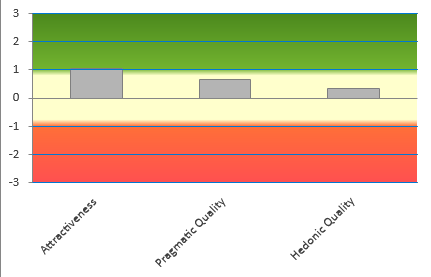
\includegraphics[width=\linewidth]{./Screenshots/Attractiveness_Pragmatic_Hedonic_Quality.png}
		\captionof{figure}{The Attractiveness, Pragmatic and Hedonic Quality}
		\label{fig:Attractiveness_Pragmatic_Hedonic_Quality}
	\end{figure}
	\par
	\newpage
	
	\printbibliography % Output the bibliography
\end{document}
